\section{Einleitung}

\subsection{Informationstheorie}

\subsection{Quellcodierung}

\section{Blockcodes}

\section{Galois-Felder}
\label{sec:galois}

%% addiitve inverse
%% multiplikative inverse
%% modulare inverse (= multiplikative inverse mod n)

\section{Reed-Solomon-Code}

$n$: Länge Codewort\\
$k$: Länge Informationswort\\
$d$: Mindestabstand

\subsection{Wunsch und Idee}

\textbf{Wunsch}

Konstruktion eines Codes mit vorgegebener Korrekturfähigkeit\\
$\rightarrow$ Vorgabe des Mindestabstandes $d$

$\displaystyle{
    e = \Bigl\lfloor \frac{d - 1}{2} \Bigr\rfloor
}$\\
$\displaystyle{
    d = 2e - 1
}$

bei linearem Code ist Mindestabstand = Mindestgewicht

$\rightarrow$ Codeworte haben mind. $d$ von 0 verschiedene Koeffizienten

d'Alembert: Polynom vom Grad $n$ hat $n$ komplexe (oder höchstens $n$ reelle) Nullstellen; auch
im Galois-Feld

\textbf{Idee}

Konstruktion des Informationswortes als Polynom $A(x)$ mit Grad $k-1$ (damit höchstens $k-1$ Nullstellen)

Im $GF(p)$ mit Ordnung $n = p-1$ kann man $A(x)$ an $n$ Stellen auswerten, danach wiederholen sich die Werte

$\rightarrow$ Auswertung des Polynoms für verschiedene $x$ (bzw. $\alpha^i$) ergeben die Koeffizienten $a_i$ des
Polynoms $a(x)$

$\displaystyle{
    a_i = A(\alpha^i) \qquad\qquad \text{IDFT}
}$

von diesen sind höchstens $k-1$ Null (weil $grad(A(x)) = k-1$)\\
von diesen sind also mind. $n - (k-1)$ von Null verschieden $\rightarrow$ Mindestgewicht $d$

$d = n - (k - 1) = n - k + 1$

\subsection{Codierung}

Verschiedene Möglichkeiten aus einem Informationswort ein Codewort zu generieren

\subsubsection{IDFT (nicht systematisch)}

$\displaystyle{
    a_i = A(\alpha^i)
}$

$A(x)$: Informationswort\\
$a_i$: Koeff. des Codewortes

\subsubsection{Generatorpolynom (nicht systematisch)}

$\displaystyle{
    a_i = g(x) \cdot i(x)
}$

mit Generatorpolynom

$g(x) = \prod_{i=k}^{n-1} (x - \alpha^{-i})$

$g(x)$: Generatorpolynom\\
$i(x)$: Informationspolynom

\subsubsection{Polynomdivision (systematisch)}

Informationswort ist Teil des Codewortes (an den hohen Potenzen)

$\displaystyle{
    a^*(x) = i_{k-1} x^{n-1} + i_{k-2} x^{n-2} + ... + i_1 x^{n-k+1} + i_0 x^{n-k}
}$

jedes Codewort muss durch Generatorpolynom teilbar sein $\rightarrow$ ist
für $a^*(x)$ i.A. nicht der Fall

$\displaystyle{
    \frac{a^*(x)}{g(x)} = b(x) + \frac{rest(a^*(x))}{g(x)}
}$\\
$\displaystyle{
    \rightarrow \frac{a^*(x) - rest(a^*(x))}{g(x)} = b(x)
}$\\
$\displaystyle{
    a(x) = a^*(x) - rest(a^*(x))
}$

$rest(a^*(x))$: Divisionsrest

\subsubsection{Über Prüfpolynom (systematisch)}

Prüfpolynom:

$\displaystyle{
    h(x) = \prod_{i=0}^{k-1} (x - \alpha^{-i})
}$

Produkt aus Generator- und Prüfpolynom ist 0

$\displaystyle{
    g(x) \cdot h(x) = 0
}$

\subsection{Decodierung}

\textbf{Idee:}

Addition des Fehlerpolynoms $f(x)$ mit $t$ Koeffizienten (d.h. $t$ Fehler sind auf dem Kanal aufgetreten)
zum gesendeten Codewort $a(x)$

im Zeitbereich:

$\displaystyle{
    r(x) = a(x) + f(x)
}$

im Frequenzbereich:

$\displaystyle{
    R(x) = A(x) + F(x)
}$

gedanklich wird ein Polynom $c(x)$ aufgestellt, welches $t$ Nullen an den Fehlerstellen hat

Da die Koeffizienten von $c(x)$ die Auswertung ihrer Fouriertransformierten $C(x)$ ist, ist der Grad
von $C(x)$ $t$

Da $c(x)$ gerade dort 0 ist, wo $f(x)$ ungleich 0, ist das Produkt $f_i \cdot c_i$ immer 0 (Achtung, keine
Polynommultiplikation gemeint, sondern punktweise Multiplikation)

$\displaystyle{
    f_i \cdot c_i = 0
}$

wenn Zeitbereich = 0 $\rightarrow$ Frequenzbereich = 0

$\displaystyle{
    F(x) \cdot C(x) = 0
}$

Achtung: hier Polynommultiplikation/ Faltung/ Filterung gemeint\\
$\hookrightarrow$ Aufstellen der Schlüsselgleichungen

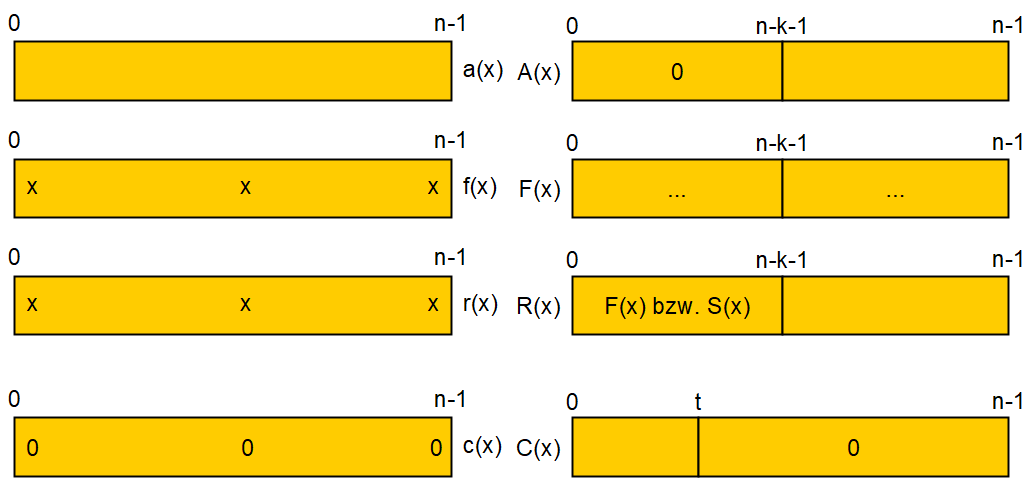
\includegraphics[width=8cm]{img/decod_rs.PNG}

\textbf{Schlüsselgleichungen}

beschreiben, dass Faltung von $C(x)$ und $F(x)$ Null sind (Achtung: zyklische Faltung, siehe \autoref{sec:galois})

$F_0$ bis $F_{n-k-1}$ (bzw. $F_{d-2}$) sind bekannt, da diese direkt an den Syndromstellen
von $R(x)$ stehen

Alle $C$-Koeff. sind unbekannt, außer $C_{t-1}$, dieser wird zu $1$ gesetzt\\

$\displaystyle{
    C_{t-1} = 1
}$

da Anzahl der Fehler ($t$) unbekannt sind, muss ausprobiert werden, welche minimale Anzahl an Fehlern
die Schlüsselgleichungen erfüllt



\subsection{Horner-Schema}

\section{Erweiterungskörper}

Erweitern des Grundkörpers (z.B. $2$) mit Exponent (z.B. $4$) $\rightarrow$
$GF(2^4)$

primitives Element wird zu primitivem Polynom, z.B.
$\displaystyle{
    p(x) = x^4 + x + 1
}$

\section{BCH-Codes}

